\documentclass[9pt]{beamer} 
\usetheme{cwc} 

\usepackage{amsmath,amssymb}
\usepackage{graphicx,acronym,setspace,epstopdf}
\usepackage[ruled]{algorithm2e}
\usepackage{subeqnarray,multirow,cite,array,color,mathtools,setspace,geometry}

\acrodef{MSE}{mean squared error}
\acrodef{BC}{broadcast channel}
\acrodef{MC}{multi-cell}
\acrodef{BS}{base station}
\acrodef{MIMO}{multiple-input multiple-output}
\acrodef{SISO}{single-input single-output}
\acrodef{MU}{multi-user}
\acrodef{MU-MIMO}{\acl{MU} \acl{MIMO}}
\acrodef{OFDM}{orthogonal frequency division multiplexing}
\acrodef{WSRM}{weighted sum rate maximization}
\acrodef{QoS}{quality of service}
\acrodef{SCA}{successive convex approximation}
\acrodef{SNR}{signal-to-noise ratio}
\acrodef{MMSE}{minimum \acl{MSE}}
\acrodef{SIR}{signal-to-interference ratio}
\acrodef{SINR}{signal-to-interference-plus-noise ratio}
\acrodef{Q-WSRM}{queue \acl{WSRM}}
\acrodef{QM}{queue minimizing}
\acrodef{SRA}{spatial resource allocation}
\acrodef{JSFRA}{joint space-frequency resource allocation}
\acrodef{WMMSE}{weighted \acl{MMSE}}
\acrodef{KKT}{Karush-Kuhn-Tucker}
\acrodef{GP}{geometric programming}
\acrodef{SOC}{second-order cone}
\acrodef{BCDM}{block coordinate descent method}

\newcommand{\mbf}[1]{\mathbf{#1}}
\newcommand{\me}[1]{\( #1 \)}
\newcommand{\mc}[1]{\mathcal{#1}}
\newcommand{\fall}{\forall}
\newcommand{\set}[1]{\left \lbrace #1 \right \rbrace }
\newcommand{\mvec}[2]{\mathbf{#1}_{#2}}
\newcommand{\ith}[1]{{#1}^\mathrm{th}}
\newcommand{\pr}[1]{{#1}^\prime}
\newcommand{\mbfa}[1]{{\boldsymbol{#1}}}
\newcommand{\herm}{\mathrm{H}}
\newcommand{\sset}[1]{\left [ #1 \right ]}
\newcommand{\rfrac}[2]{{}^{#1}/{}_{#2}}
\newcommand{\eqspace}{\IEEEeqnarraynumspace}
\newcommand{\enoise}{\widetilde{N}_0}
\newcommand{\eqsub}{\IEEEyessubnumber}
\newcommand{\review}[1]{{\textcolor[rgb]{0 0 0.6}{#1}}}
\newcommand{\trace}{\mathrm{tr}}
\newcommand{\tran}{\mathrm{T}}
\newcommand{\R}[1]{\label{#1}\linelabel{#1}}
\newcommand{\lr}[1]{page~\pageref{#1}, line~\lineref{#1}}
\newcommand{\eqn}[1]{\(#1\)}
\newcommand{\mx}{\mbf{m}}
\newcommand{\my}{\mbf{w}}
\newcommand{\mz}{\mbfa{\gamma}}
\newcommand{\mxb}{{{\mbf{m}}}}
\newcommand{\myb}{{{\mbf{w}}}}
\newcommand{\iterate}[2]{{#1}^{(#2)}}
\newcommand{\iter}[3]{{#1}_{#2}^{(#3)}}
\newcommand{\ma}{\mbf{x}}
\acrodef{MSE}{mean squared error}
\acrodef{IBC}{interference broadcast channel}
\acrodef{MC}{multi-cell}
\acrodef{BS}{base station}
\acrodef{MIMO}{multiple-input multiple-output}
\acrodef{SISO}{single-input single-output}
\acrodef{MU}{multiple users}
\acrodef{OFDM}{orthogonal frequency division multiplexing}
\acrodef{WSRM}{weighted sum rate maximization}
\acrodef{QoS}{quality of service}
\acrodef{SCA}{successive convex approximation}
\acrodef{SNR}{signal-to-noise ratio}
\acrodef{MMSE}{minimum \acl{MSE}}
\acrodef{SIR}{signal-to-interference ratio}
\acrodef{SINR}{signal-to-interference-plus-noise ratio}
\acrodef{Q-WSRM}{queue \acl{WSRM}}
\acrodef{QM}{queue minimizing}
\acrodef{SRA}{spatial resource allocation}
\acrodef{JSFRA}{joint space-frequency resource allocation}
\acrodef{WMMSE}{weighted \acl{MMSE}}
\acrodef{KKT}{Karush-Kuhn-Tucker}
\acrodef{GP}{geometric programming}
\acrodef{SOC}{second-order cone}
%\acrodef{BCDM}{block coordinate descent method}
\acrodef{ADMM}{alternating directions method of multipliers}
\acrodef{PD}{primal decomposition}
\acrodef{DD}{dual decomposition}
\acrodef{FFR}{fractional frequency reuse}
\acrodef{DC}{difference of convex}
\acrodef{Q-WSRME}{\ac{Q-WSRM} extended}
\acrodef{TDD}{time division duplexing}
\acrodef{CSI}{channel state information}
\acrodef{AO}{alternating optimization}
\acrodef{OTA}{over-the-air}
\acrodef{PL}{path loss}
\acrodef{TDM}{time division multiplexing}
\acrodef{UC}{uncoordinated}

\graphicspath{{./../Figures/}{./../Figures/Linux/}{./../Figures/Review/}}
\DeclareGraphicsExtensions{.eps}

\epstopdfsetup{update,prepend,prefersuffix=false,suffix=}
\DeclareGraphicsRule{.eps}{pdf}{.pdf}{`epstopdf #1}
\pdfcompresslevel=9

\linespread{1.4}

\title{Traffic Aware Precoder Design for Space Frequency Resource Allocation}
\author{{Ganesh Venkatraman, Antti T\"{o}lli, Le-Nam Tran and Markku Juntti\eqn{^\dagger}} \\ \scriptsize{Email: \{gvenkatr, antti.tolli, le.nam.tran, markku.juntti\}@ee.oulu.fi}}


\begin{document}

\AtBeginSection{\frame{\sectionpage}}

\begin{frame}
    \titlepage
\end{frame}

\begin{frame}{Outline} \scriptsize
    \tableofcontents
\end{frame}

\acused{BS} \acused{MIMO} \acused{OFDM}

\section{Introduction}

\begin{frame}{Introduction and Motivation}
\begin{itemize}
\item Complex algorithms are adopted to maximize throughput to satisfy the data requirements from higher layers
\item Available wireless resources are to be utilized efficiently to minimize the backlogged packets 
\item Spatial and Frequency resources are exploited to empty the packets waiting at the \acp{BS}
\item In this work, we discuss precoder designs for \acl{MU} \acs{MIMO}-\acs{OFDM} setup to minimize the number of queued packets 
\end{itemize}
\end{frame}

\section{System Model \& Problem Formulation}

\begin{frame}{Symbols used}
\begin{itemize}
\item \acs{OFDM} system with \me{N} sub-channels and \me{N_B} \acp{BS}, each equipped with \me{N_T} transmit antennas
\item Let \me{K} be the total number of users with \me{N_R} antennas
\item Let \me{\mc{B}} and \me{\mc{U}} denote the set of coordinating \acp{BS} and users in the system
\item The set of users belonging to \acs{BS} \me{b} is denoted by \me{\mc{U}_b \in \mc{U}}
\item Let \me{b_k \in \mathcal{B}} denotes the \ac{BS} serving the user \me{k}
\item Let \me{L} be the total available spatial streams for a user \me{k}, given by \me{\min (N_T,N_R)}
\end{itemize}
\end{frame}

\begin{frame}{System Model}
\begin{itemize}
\item The \me{\ith{l}} spatial signal received on sub-channel \me{n} of user \me{k} is given by
\begin{multline}\label{eqn-1}
\hat{d}_{l,k,n} = \mvec{w}{l,k,n}^\herm \mvec{H}{b_k,k,n} \,\mvec{m}{l,k,n} d_{l,k,n} + \mvec{w}{l,k,n}^\herm \mvec{n}{l,k,n} \\ 
+ \mvec{w}{l,k,n}^\herm \sum_{i \in \mc{U} \backslash \set{k}} \mvec{H}{b_i,k,n} \sum_{j = 1}^L \mvec{m}{j,i,n}d_{j,i,n}
\end{multline}
\item where \me{\mvec{m}{l,k,n}} and \me{\mvec{w}{l,k,n}} are transmit and receive beamformers corresponding to the \me{\ith{l}} spatial stream on the \me{\ith{n}} sub-channel of user \me{k}
\end{itemize}
\end{frame}

\begin{frame}{System Model}
\begin{itemize}
\item \me{\mvec{H}{b_k,k,n} \in \mathbb{C}^{N_R \times N_T}} denotes the channel between \ac{BS} \me{b_k} and user \me{k}
\item \me{d_{l,k,n}} and \me{{n}_{l,k,n}} correspond to data symbol and equivalent noise on \me{\ith{l}} spatial stream of user \me{k}
\item Using the above notations, the \acs{SINR} seen by the \me{\ith{l}} spatial stream on the \me{\ith{n}} sub-channel for user \me{k} is given by
\end{itemize}
\begin{equation}\label{eq:SINR}
\gamma_{l,k,n} = \dfrac{\left |\mvec{w}{l,k,n}^\herm \, \mvec{H}{b_k,k,n} \, \mvec{m}{l,k,n} \right |^2}{\enoise + \sum_{(j,i) \neq (l,k)} |\mvec{w}{l,k,n}^\herm \mvec{H}{b_i,k,n} \mvec{m}{j,i,n} |^2}
\end{equation}
\begin{itemize}
\item where \eqn{\enoise = \|\mvec{w}{l,k,n}^\herm \mvec{n}{l,k,n} \|^2 }
\end{itemize}
\end{frame}

\begin{frame}{Queueing Model}
\begin{itemize}
\item Each user is associated with backlogged packets of size \me{Q_k} packets.
\item Queued packets \me{Q_k} of each user follows dynamic equation at the \me{\ith{i}} instant as
\begin{equation}
Q_k(i+1) = \Big [ Q_k(i) - t_k(i) \Big ]^+ + \lambda_k(i)
\label{eqn-2a}
\end{equation}
\item where \me{t_k = \sum_{n = 1}^N \, \sum_{l = 1}^L \, t_{l,k,n}} denotes the total number of transmitted packets corresponding to user \me{k} in the previous \me{\ith{i}} instant
\item \me{\lambda_k} represents the fresh arrivals of user \me{k} at \ac{BS} \me{b_k}
\end{itemize}
\end{frame}

\begin{frame}{Problem Formulation}
\begin{itemize}
\item Available spatial and frequency resources are to be efficiently utilized to minimize the queued packets
\item {\color{red}Objective} - to minimize the number of backlogged packets waiting at \acp{BS}
\item {\color{red}Optimization variables} - transmit precoders and receive beamformers
\item {\color{red}\ac{MIMO}-\ac{OFDM}} - scheduling of users across sub-channels is inherently performed by precoders
\end{itemize}
\end{frame}

\section{Centralized Solutions}

\subsection{Existing \acs{Q-WSRM} Formulation}

\begin{frame}{Queue-Weighted Sum Rate Maximization (\acs{Q-WSRM})}
\begin{itemize}
\item \acs{Q-WSRM} formulation is the result of minimizing the conditional Lyapunov drift\eqn{^\dagger}
\item \acs{Q-WSRM} formulation is also called as back pressure algorithm, since it acts greedily in minimizing the backlogged packets at each instant
\[ \underset{t_{l,k,n}}{\text{minimize}} \quad \sum_{k \in \mc{U}} \left \lbrace Q_k(i)^2 - Q_k(i-1)^2 \right \rbrace, \]
\item where \me{Q_k} follows the dynamic Queue expression in \eqref{eqn-2a} and \me{t_k = \sum_{n = 1}^N \, \sum_{l=1}^L \, t_{l,k,n}}
\end{itemize}

\vspace{2eM}
\eqn{^\dagger}\footnotesize{Neely, Michael J. "Stochastic network optimization with application to communication and queueing systems." Synthesis Lectures on Communication Networks 3.1 (2010): 1-211.}
\end{frame}

\begin{frame}{Queue-Weighted Sum Rate Maximization (\acs{Q-WSRM})}
\begin{itemize}
\item \acs{Q-WSRM} formulation, which is obtained by solving Lyapunov drift, is given by
\end{itemize}
\begin{subequations}
\begin{align}
 \underset{t_{l,k,n}}{\text{maximize}} & \qquad \sum_{k \in \mc{U}} \; Q_k \left ( \alert{\sum_{n=1}^N} \, \sum_{l = 1}^L  t_{l,k,n} \right ) \\
& \qquad {\color{blue} \alert{\sum_{n=1}^N} \, \sum_{l = 1}^L  t_{l,k,n}  \leq \alert{Q_k} \; / \; Q_{k,n}}
\end{align}
\end{subequations}
\begin{itemize}
\item Queue-Rate product is maximized
\item Users with more number of backlogged packets are favored over good channel users
\end{itemize}
\end{frame}

\begin{frame}{Queue-Weighted Sum Rate Maximization (\acs{Q-WSRM})}
	\begin{itemize}
		\item Complexity can be reduced if precoders are designed for each sub-channel independently
		\item Coupling across sub-channels is obtained by the queues, which are updated after evaluating the rate from previously chosen sub-channels as
	\end{itemize}
	\begin{equation*}
	Q_{k,n} = \max{\Big \lbrace Q_k - \sum_{j = 1}^{n-1} \, \sum_{l = 1}^{L} \, t_{l,k,j} ,0 \Big \rbrace }, \; \forall \; k \in \mathcal{U}
	\end{equation*}
\end{frame}

\subsection{\acs{JSFRA} Formulation (\acs{SINR} Relaxation)}

\begin{frame}{\acs{JSFRA} Formulation (\acs{SINR} Relaxation)}
\begin{itemize}
\item Precoders are designed by a centralized controller, which are then used by all \acp{BS} in \me{\mc{B}}
\item The objective used to design transmit precoders is 
\begin{equation}
\scriptsize {\color{blue} v_k = \left | Q_k - \sum_{n = 1}^N \sum_{l = 1}^{L} t_{l,k,n} \right |^q }
\end{equation}
\item To generalize the objective, we use \me{\tilde{v}_k \triangleq a_k^{\frac{1}{q}} \, v_k}, where \me{a_k} is arbitrary weights used control the priorities
\item Exponent \me{q} plays different role based on the value it assumes
	\begin{itemize}
	\item \me{\ell_{q=1}} results in greedy allocation
	\item \me{\ell_{q=2}} ideal for the delay or buffer size limited scenarios
	\item \me{\ell_{q=\infty}} provides fair resource allocation in each transmission instant
	\end{itemize}
\end{itemize}
\end{frame}

\begin{frame}{\acs{JSFRA} Formulation (\acs{SINR} Relaxation)}
\begin{itemize}
\item Optimization problem with queue difference objective is nonconvex due to the constraint
\begin{equation}  \scriptsize
\alert{\gamma_{l,k,n} \leq \dfrac{\left |\mvec{w}{l,k,n}^H \, \mvec{H}{b_k,k,n} \, \mvec{m}{l,k,n} \right |}{\beta_{l,k,n}}^2 }
\end{equation}
\item The nonconvex constraints are approximated by sequence of convex subsets and solved iteratively
\item Convergence of the iterative algorithm is guaranteed
\item Receive beamformers are designed by the \acs{MMSE} receivers using the converged transmit precoders
\end{itemize}
\end{frame}

\subsection{\acs{JSFRA} Formulation (\acs{MSE} Reformulation)}

\begin{frame}{\acs{JSFRA} Formulation (\acs{MSE} Reformulation)}
	\begin{itemize}
	\item Alternatively, we solve the queue minimization problem by utilizing the relation between the \acs{MSE} and the \acs{SINR} as \me{\color{blue} \epsilon_{l,k,n} = (1 + \gamma_{l,k,n})^{-1}}
	\item Equivalence is valid only when the receivers are designed with the \ac{MSE} objective, \textit{i.e.}, using \acs{MMSE} receivers
	\begin{eqnarray} \label{mse-error} \scriptsize
	\mathbb{E} \big [ ( d_{l,k,n} - \hat{d}_{l,k,n} )^2 \big ] = \big | 1 - \mvec{w}{l,k,n}^\herm \mvec{H}{b_k,k,n} \mvec{m}{l,k,n} \big |^2 \nonumber \\
	+ \sum_{{(j,i) \neq (l,k)}} \big | \mvec{w}{l,k,n}^\herm \mvec{H}{b_i,k,n} \mvec{m}{j,i,n} \big |^2 + \enoise = \epsilon_{l,k,n}
	\end{eqnarray}
	\item Problem involves nonconvex constraint 
	\begin{equation}
	\alert{t_{l,k,n} \leq -\log_2(\epsilon_{l,k,n})}
	\end{equation}
	\end{itemize}
\end{frame}

\begin{frame}{\acs{JSFRA} Formulation (\acs{MSE} Reformulation)}
	\begin{itemize}
		\item The nonconvex constraint is approximated by a sequence of convex constraints
		\item It is achieved by using \ac{SCA} technique
		\item The iterative procedure is performed until convergence or for suitable number of iterations
		\item \alert{The above reformulation works only with the \acs{MMSE} receiver}
	\end{itemize}
\end{frame}

\section{Distributed Solutions}

\subsection{Primal \& \acs{ADMM} based decompositions}

\begin{frame}{Distributed Methods}
	\begin{itemize}
		\item Small System - centralized approach is viable, provided channel remains constant for multiple transmission slots
		\item However, overhead involved in the centralized design scales up significantly as the network size grows
		\item Distributed approaches based on primal decomposition or \acs{ADMM} can be used to reduce the signaling requirements
		\item Overhead involved in the design of precoders are only scalar interference variables
		\item Only convex approximated subproblem in each \acs{SCA} step is performed via distributed approaches
	\end{itemize}
\end{frame}

\begin{frame}{Primal Decomposition Method}
	\begin{itemize}
		\item Precoder design is based on master-slave approach
		\item Interference to the neighboring \ac{BS} users are bounded by a scalar variable
		\item The interference thresholds are determined by the master problem and used in each slave subproblem constraint as
		\begin{equation} \label{inter_exp} \scriptsize
		\zeta_{l,k,n,b} \geq \sum_{i \in \mc{U}_b} \sum_{j = 1}^L |\mvec{w}{l,k,n}^\herm \mvec{H}{b,k,n} \mvec{m}{j,i,n} |^2 \; \forall b \in \bar{\mc{B}}_{b_k}.
		\end{equation}
	\end{itemize}
\end{frame}

\acused{ADMM}
\begin{frame}{ADMM based Decomposition Method}
	\begin{itemize}
		\item The \ac{ADMM} is superior to other distributed schemes in terms of the convergence speed
		\item \ac{ADMM} includes an additional quadratic term 
		\begin{equation}
		\color{blue} \|v_k\|_q + \sum_{l,k,n} \nu_{l,k,n}^{(j)} \left ( \mbfa{\zeta}_b - \mbfa{\zeta}^{(j)}_b \right ) + \frac{\rho}{2}  \| \mbfa{\zeta}_b - \mbfa{\zeta}^{(j)}_b \|^2
		\end{equation}
		in objective, where \eqn{\mbfa{\zeta}^{(j)}_b} is global consensus variable
		\item \eqn{\zeta_{l,k,n,b}} in \eqref{inter_exp} is treated as an optimization variable in \ac{ADMM}
		\item The consensus variables are updated as
		\begin{equation} \scriptsize
		\mbfa{\zeta}_{b_k}(b)^{(j+1)} = \mbfa{\zeta}_{b}(b_k)^{(j+1)} = \frac{\mbfa{\zeta}_{b}(b_k) + \mbfa{\zeta}_{b_k}(b)}{2}
		\end{equation}
		\item where \eqn{\mbfa{\zeta}_{b_k}(b)} denotes the entries corresponding to \ac{BS} \eqn{b} in \ac{BS} \eqn{b_k}
	\end{itemize}
\end{frame}

\subsection{KKT based Distributed Solution}

\begin{frame}{KKT based Distributed Solution}
	\begin{itemize}
		\item Decentralization methods considered so far involve considerable signaling exchanges via backhaul
		\item Since the overhead involved is large for multi-antenna receivers, the iterative design should reduce the backlogged packets significantly in first few iterations
		\item To achieve that, we design an iterative procedure by solving the \ac{KKT} equations of the \acs{JSFRA} problem via \acs{MSE} reformulation
		\item Group update of all the involved optimization variables is carried out to speed up the convergence of precoder design
	\end{itemize}
\end{frame}

\section{Simulation Results}

\subsection{Centralized Solutions}

\begin{frame}{Centralized Solutions}
\begin{figure}
	\centering
	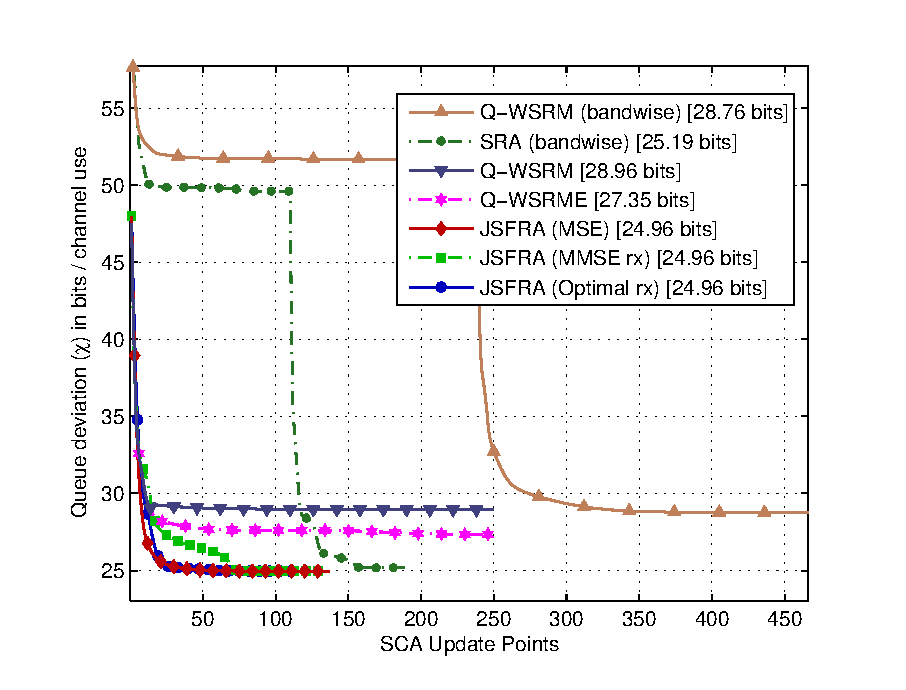
\includegraphics[width=0.75\textwidth]{fig-2-5}
	\caption{System Model - \me{\lbrace N,N_B,K,N_T,N_R \rbrace = \lbrace 2,3,9,4,2\rbrace}}
\end{figure}
\end{frame}

\subsection{Distributed Solutions}

\begin{frame}{Distributed Solutions}
	\begin{figure}
		\centering
		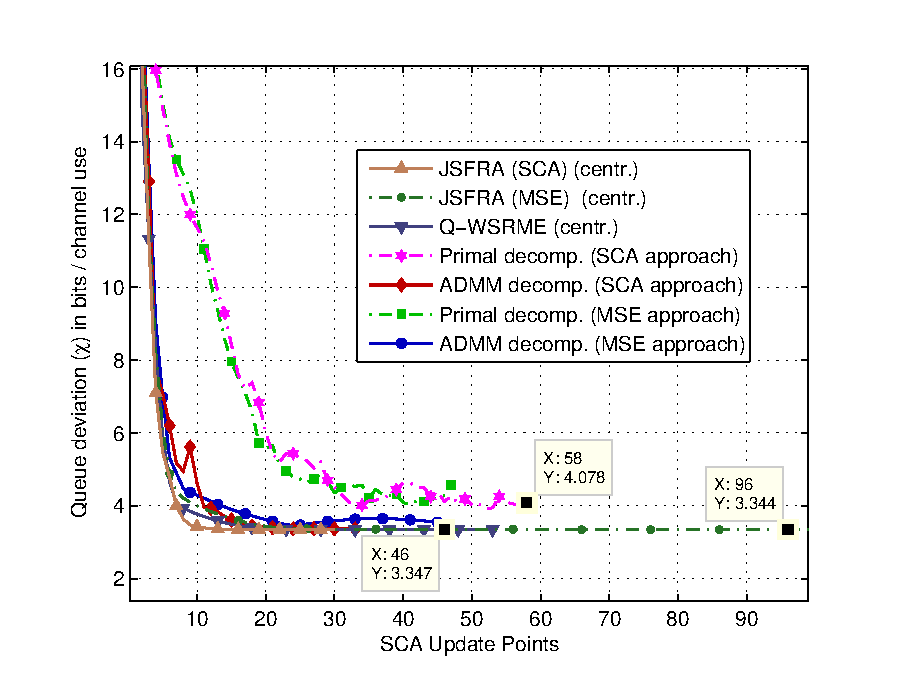
\includegraphics[width=0.75\textwidth]{fig-3-2}
		\caption{System Model - \me{\lbrace N,N_B,K,N_T,N_R \rbrace = \lbrace 3,2,8,4,1 \rbrace}}
	\end{figure}
\end{frame}

\subsection{KKT based Approach}

\begin{frame}{Performance of KKT based Approach}
	\begin{figure}
		\centering
		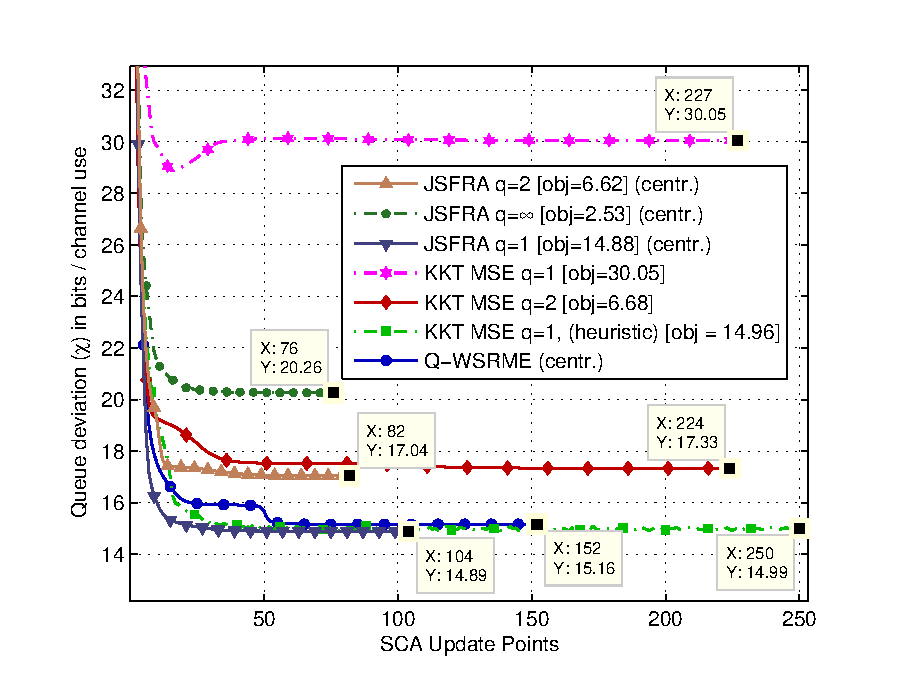
\includegraphics[width=0.75\textwidth]{fig-9-3}
		\caption{System Model - \me{\lbrace N,N_B,K,N_T,N_R \rbrace = \lbrace 5,2,8,4,1 \rbrace}}
	\end{figure}
\end{frame}

\subsection{Time Correlated Fading Performance}

\begin{frame}{Time Correlated Fading Performance}
	\begin{figure}
		\centering
		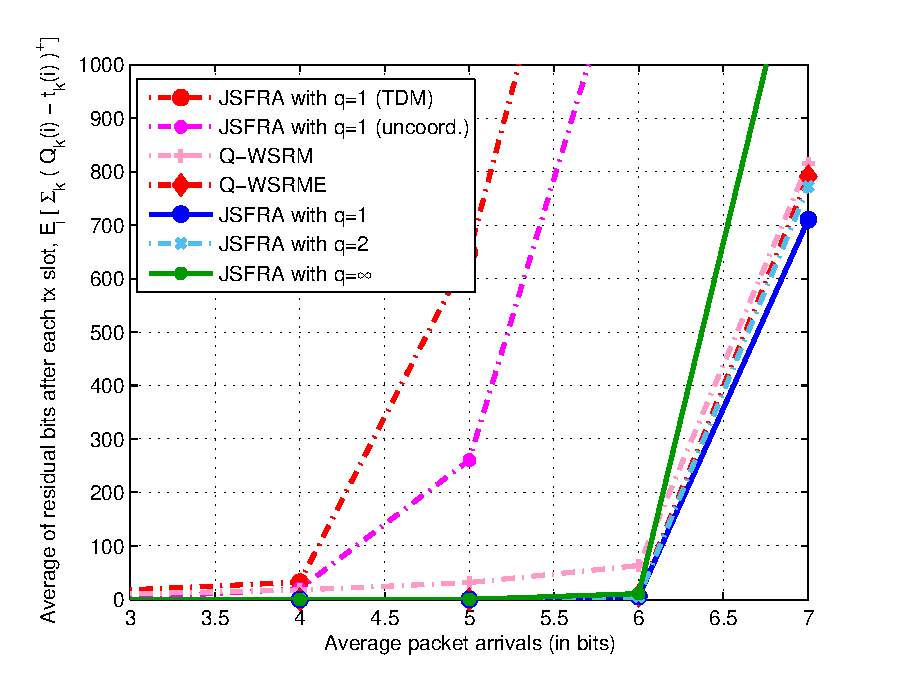
\includegraphics[width=0.75\textwidth]{average_queue_over_time-3}
		\caption{System Model - \me{\lbrace N,N_B,K,N_R \rbrace = \lbrace 3,2,8,1 \rbrace} after \eqn{250} transmissions}
	\end{figure}
\end{frame}

\section{Conclusions}

\begin{frame}{Conclusions}
\begin{itemize}
\item We discussed the problem of wireless resource allocation to minimize backlogged packets in an efficient way
\item The proposed approach uses \ac{SCA} method by using linear approximation for the nonconvex constraint
\item We also addressed different distributed methods for the precoder design across each \acsp{BS} with minimal information exchange
\item An iterative algorithm for the \acs{JSFRA} scheme using \acs{MSE} reformulation is also studied
\end{itemize}
\end{frame}


\begin{frame}
\begin{center}
{\color{blue}\Huge{Questions !}}
\end{center}
\end{frame}

\end{document}
